\chapter{序論}

\section{X線CTとは}
X線CT(Computed Tomography)は、医療用画像診断装置の一種で、人体を切開することなく内部の状態を立体的に観察することができる装置である(\Fref{fig:gaikan}(左))。レントゲン撮影と同様にX線を用いて透過写真を得るが、レントゲン写真では三次元の被写体が二次元映像として表されるのに対し、CTでは多数の向きからX線撮影を行うことで、内部の状態を立体的に表現することが可能である。CTでしか見つからない体内の病変は大変多く、X線CTは現在の医療画像診断においても根幹をなす重要技術であるといえる。その原理はX線を人体に向かって照射し、その透過強度を検出器で測定し、X線の通しにくさを表した投影データを取得し画像再構成をすることによってCT画像を再構成している。検出器にはシンチレータとフォトダイオードが用いられており、シンチレータでX線を光に変換し、フォトダイオードで光電変換を行い読み出すのが現在のCTの主流である。
\vspace{0.5cm}
\begin{figure}[H]
 \begin{minipage}{0.5\hsize}
  \begin{center}
  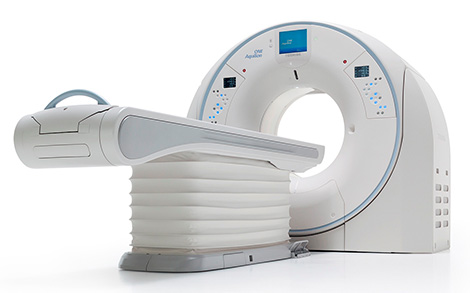
\includegraphics[bb=0.000000 0.000000 470.000000 293.000000,width=0.9\hsize]{image2/chapter1/toshibaCT.jpg} 
  \end{center}
  \vspace{-1cm}
  \caption*{}
 \end{minipage}
 \begin{minipage}{0.5\hsize}
  \begin{center}
 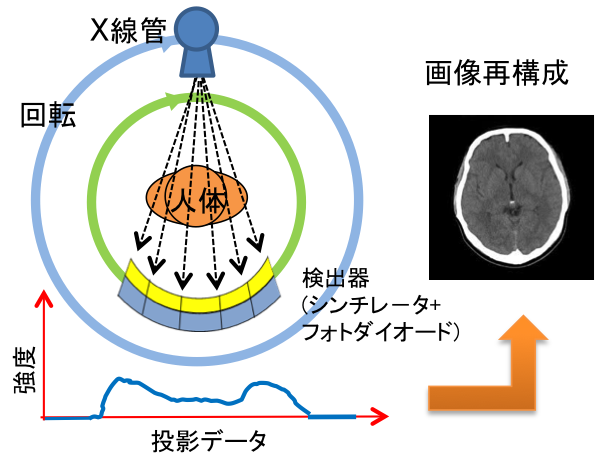
\includegraphics[bb=0.000000 0.000000 287.496234 222.221630,width=0.9\hsize]{image2/chapter1/CT_genri.png} 
  \end{center}
  \vspace{-1cm}
  \caption*{}
 \end{minipage}
 \begin{center}
  \caption{(左)X線CTの外観と(右)X線CTの原理}
  \label{fig:gaikan}
  \end{center}
\end{figure}


\section{従来のX線CTの問題点}
フォトダイオードの暗電流は 数十pA$\sim$数百pAであり、この暗電流に十分打ち克つ信号電流を検出器から出力する必要がある。CTの画質を律速しているのは「信号電流($I_s$)$\gg$暗電流($I_d$)」を実現することに他ならない。ここで従来のCTにおいて「$I_s\gg I_d$」を実現させるために必要な照射線量を概算してみる。被写体透過後のX線強度を$I_x$[/s]、PDの暗電流$I_d$を100[pA]とする。60keVのX線が従来一般的に用いられるGOSシンチレータ(40,000 ph/MeV)に検出されたとし、PDの量子効率を50\%すると、

\begin{align}
I_d&\gg I_s\\
60\time40\times0.5\times1.6\times10^{-19} [C] \times I_x&\gg100\times10^{-12}\\
I_x&\gg 5.2\times10^5
\end{align}
程度となる。また読み出し回路を通ることでさらにノイズが増大することを考えれば被写体を透過した時点で$10^{6}$cts/s/mm$^2$のレートが必要になる。人体透過後は線量は約1/1000になるので\footnote{人体を水と透過と考え60keVにおける水の線減弱係数は0.206[1/cm]、人体を30cmとすれば$e^{-\mu L}\sim1/1000$となる。}必要な照射線量は$10^{8-9}$cts/s/mm$^2$と膨大になる。このためX線CTによる医療被ばく量は膨大であり一回の撮影での被ばく量は10mSvにもおよびこれは成人の年間被ばく量の5倍に相当する\Fref{fig:dose}(左)。また日本においてはCTの普及率が世界1位であるため\Fref{fig:dose}(右)、国民一人あたりの医療被ばく量が諸外国に比べて圧倒的に高い。特に子どもや妊婦においては発がんリスクが高まることが報告されておりCTの適用が制限されている。日本においてはこれから高齢者人口が増えCTの需要はさらに高まり、このCTによる医療被ばくの問題は増々深刻化すると考えられる。

また超高線量下おいては様々なエネルギーの混ざった混合エネルギーのX線のそれぞれの反応パルスイベントを区別するのは困難であり、読み出し方法はある一定時間電荷を積分した電流モードである。そのため個々のX線光子のエネルギー情報は完全に失われてしまう。そのため得られる画像はCT値のみをパラメーターとしたモノクロ画像となってしまうため、CT値が同一の物質の弁別が困難であったり、ビームハードニングアーチファクトが発生してしまうのが二点目の問題である。\\
このような背景から「低被ばく」かつ「多色」X線CTの必要性が高まっている。


\begin{figure}[H]
 \begin{minipage}{0.5\hsize}
  \begin{center}
 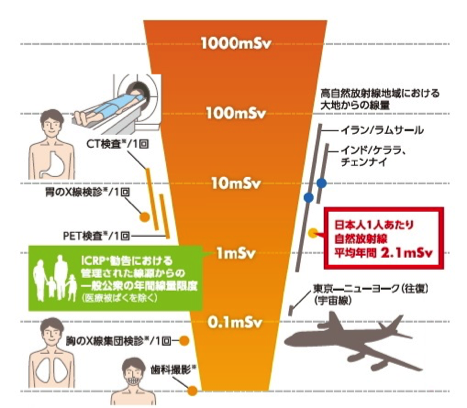
\includegraphics[bb=0.000000 0.000000 224.141471 195.823812,width=0.9\hsize]{image2/chapter1/dose_medical.png} 
  \end{center}
  \vspace{-1cm}
  \caption*{}
 \end{minipage}
 \begin{minipage}{0.5\hsize}
  \begin{center}
 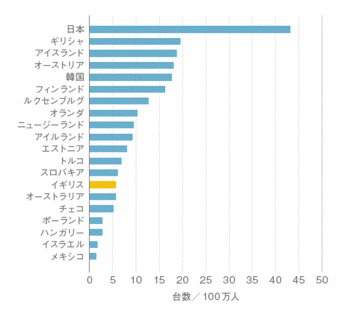
\includegraphics[bb=0.000000 0.000000 350.000000 313.000000,width=0.9\hsize]{image2/chapter1/CT_number.png} 
  \end{center}
  \vspace{-1cm}
  \caption*{}
 \end{minipage}
 \begin{center}
  \caption{(左)自然放射線と医療放射線の被ばく量比較(右)各国のCT保有台数}
  \label{fig:dose}
  \end{center}
\end{figure}



\section{各医療メーカーの新型CT}
上述のように「低被ばく」かつ「多色」X線CTの必要性が高まる中でCTメーカー各社も様々な手法でそれを実現しようとしてる。GEにおいてはASiR-VというFBPとMLEMを組み合わせた新たな画像再構成アルゴリズムを開発し従来よりも低線量でも同等の画質を保てるCTを開発している。また、X線管を回転させながら高速で管電圧を80kVと140kVを切り替えることによってデュアルエナジーCTを実現している。またPhilipsにおいてはシンチレーターを二層式にすることで、一層目で低エネルギーのX線を検出し、二層目で高エネルギーのX線を検出することで2通りのCT画像を取得するデュアルエナジーCTを製品として出している。シーメンスは90度の角度差をつけた位置にX線管を配置し、管電圧を80kVと140kVのX線を照射することにより2色のデュアルエナジーCTを実現している。

\begin{figure}[H]
 \begin{center}
 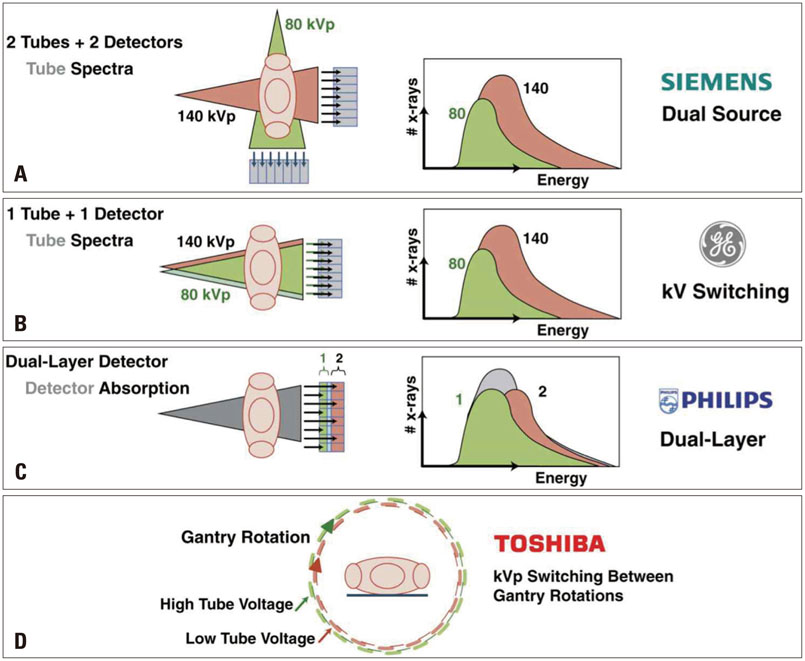
\includegraphics[bb=0.000000 0.000000 399.724138 328.220690,width=0.7\hsize]{image2/chapter1/CT_maker.jpg} 
 \end{center}
 \caption{各CTメーカーの製品化されているスペクトルCTの方式}
 \label{fig:maker}
\end{figure}

しかし、新たな画像再構成法による低被ばく化は50\%程度にとどまり、多色化は2色にとどまっているのが現状である。

\section{本研究の目的と概要}
そこで、本研究では次世代光センサーMulti-Pixel Photon Counter (MPPC)と高速シンチレータを用いて、「低被ばく」かつ「多色」撮影が可能な、全く新しい革新的X線CTシステムを提案する。MPPCは100万倍以上の大きな内部増幅機能をもつ半導体光素子で、微弱信号への感度が極めて高く「信号電流$\gg$暗電流」の特性を持つ検出器である。この大きな内部増幅により、従来型CTより遥かに低い線量で同等以上のS/Nを実現し、一方ではエネルギー弁別による多色CTも実現可能になると期待される。さらに、比較的容易に既存のCT装置と置き換えが可能と見込まれ、臨床応用へのハードルを下げることができる。本研究では最初の実証試験を行った。
本論文では、まず2章に本研究で提案するMPPCを用いたX線CTシステムの詳細を述べ、3章でPDを用いた従来型CTとの画像比較結果について述べる。4章で得られたエネルギー情報を利用したイメージング結果を示す。最後5章で、まとめと今後の展望について触れたい。






